\section{Definizione e impatto dei requisiti}
I \textbf{requisiti} di un sistema sono la descrizione dei suoi servizi e vincoli operativi; il processo della loro ricerca, analisi, documentazione e verifica è detto \textbf{ingegneria dei requisiti}. Queste caratteristiche riflettono le richieste del cliente e sono quindi orientate alla risoluzione dei suoi problemi.\par
Si tratta di una fase fondamentale del processo lavorativo, perché l'incompletezza o ambiguità dei requisiti è uno dei fattori maggiori che portano al fallimento di un progetto oppure alla sua rielaborazione, specie se in fasi avanzate dello sviluppo, con costi molto elevati. In ogni caso, definiamo due tipologie di requisiti: \begin{itemize}
	\item \textbf{Utente}: Descrizione in linguaggio naturale dei vincoli operativi e servizi forniti dal sistema. Spesso accompagnati da diagrammi per aumentarne la comprensibilità.
	\item \textbf{Di sistema}: Descrizione dettagliata e formale\footnote{Si indicano il nome della funzione, una sua descrizione, gli input, la sorgente, gli output, la destinazione, i parametri, pre-condizioni, post-condizioni, effetti collaterali e il link al requisito utente.} di funzioni, servizi e vincoli del sistema. Compone il \textbf{documento dei requisiti}, il quale specifica esattamente che cosa deve essere implementato. La sua scrittura può essere parte del contratto tra stakeholder e azienda.
\end{itemize}
\noindent È buona prassi scrivere i requisiti in più livelli di dettaglio, poiché diversi tipi di lettori li usano in modo differente. Per esempio, un receptionist che si occupa del concierge in hotel avrà bisogni differenti rispetto al manager.\par
Per scrivere un documento dei requisiti si possono usare strumenti come diagrammi UML, testi strutturati e use case. Nei metodi agili, invece, si fa spesso uso delle user stories.\newline

\begin{esempio}
	\textbf{Requisiti utente}\par
	\noindent La seguente lista puntata indica i requisiti di un software in linguaggio naturale e comprensibile per tutti:\newline
	
	\textbf{Aggiungere nodi a un design} \begin{enumerate}
		\item L'editor fornisce un mezzo per aggiungere nodi di un tipo specifico al design.
		\item La sequenza di azioni per aggiungere un nodo deve essere: \begin{enumerate}
			\item L'utente seleziona il tipo di nodo da aggiungere.
			\item L'utente muove il cursore sulla posizione del nodo approssimata nel diagramma e indicare che il simbolo del nodo dovrebbe essere aggiunto a quel punto.
			\item L'utente trascina il simbolo del nodo alla posizione finale.
		\end{enumerate}
	\end{enumerate}
\end{esempio}

\noindent I requisiti dei sistemi software sono spesso divisi anche in queste due categorie: \begin{itemize}
	\item \textbf{Requisiti funzionali}: Definizioni di servizi che il sistema deve fornire; indicano come reagisce a determinati input e come dovrebbe comportarsi nelle varie situazioni.
	\item \textbf{Requisiti non funzionali}: Vincoli su funzioni e servizi del sistema, come prestazioni, sicurezza, affidabilità o vincoli tecnologici. Includono inoltre limitazioni su tempo, processo di sviluppo e quelle richieste dagli standard. Di norma si applicano al sistema in toto e non a singole funzioni.
\end{itemize}
\begin{esempio}
	\textbf{Requisiti funzionali e non funzionali}\par
	\noindent Si consideri un sistema bancomat. I requisiti non funzionali indicano richieste indipendenti dalle funzionalità: \begin{itemize}
		\item Il sistema deve essere facilmente espandibile e adattabile alle future esigenze bancarie.
		\item Il sistema deve essere disponibile a persone portatori di Handicap, deve garantire un tempo di risposta inferiore al minuto e deve essere sviluppato su architettura X86 con sistema	operativo compatibile con quello della banca.
	\end{itemize}
	\noindent Mentre i requisiti funzionali riguardano i servizi, anche se scritti in maniera generale: \begin{itemize}
		\item Il sistema deve mettere a disposizione le funzioni di prelievo, saldo, estratto conto.
		\item Le operazioni di prelievo devono richiedere autenticazione tramite un codice segreto memorizzato sulla carta.
	\end{itemize}
\end{esempio}



%

\section{Processi di ingegneria dei requisiti}
Come già menzionato, il fine ultimo dell'ingegneria dei requisiti è il documento relativo alle funzionalità e servizi offerti dal sistema. L'attività è divisa in quattro fasi chiave: \begin{itemize}
	\item \textbf{Elicitazione dei requisiti}: Ingegneri e stakeholder lavorano insieme per studiare il dominio applicativo e definire le funzioni del sistema.\par
	Si utilizzano diverse tecniche, come le interviste, i questionari, i workshop, oppure approcci più diretti come l'osservazione sul posto di lavoro o l'analisi dei prodotti dei competitor.
	\item \textbf{Analisi dei requisiti}: Si raffinano i requisiti raccolti e si stabilisce la loro priorità\footnote{Discussione dei requisiti in termini di \textbf{must}, \textbf{could} e \textbf{should}, quindi secondo la scala MoSCow}, fattibilità e correttezza. In presenza di lacune o ambiguità, si cerca di colmarle ricavando altri requisiti o chiedendo ulteriori spiegazioni agli stakeholder.\par
	Può capitare inoltre di avere conflitti tra i requisiti; la risoluzione risiede nella negoziazione con i committenti per una modifica o rimozione della richiesta.
	\item \textbf{Specifica dei requisiti}: Processo di scrittura dei requisiti utente e di sistema in due documenti; il primo è redatto per i clienti e costituisce un contratto fra le parti, mentre il secondo è scritto per gli sviluppatori in un linguaggio tecnico e formale. Quest'ultimo rappresenta il punto di partenza per la fase di design del software.
	\item \textbf{Convalida dei requisiti}: Processo di verifica sui requisiti, per assicurarsi che descrivano il software realmente voluto dal cliente. Si cerca di sanare ogni ambiguità e confermare di avere un insieme completo per rispettare le richieste.\par
	Normalmente la convalida avviene mediante revisioni tra pari, mirando ad identificare aree di sviluppo o miglioramento. Alternativamente è possibile usare dei test case oppure sviluppare un prototipo.
\end{itemize}
\noindent Naturalmente, nelle prime fasi del lavoro si spenderanno più sforzi sulla definizione dei requisiti non funzionali, sicché siano coerenti con i desideri degli stakeholder, mentre nelle ultime fasi, appurata la loro correttezza, si potrà dare più importanza ai requisiti funzionali, per guidare al meglio il lavoro di scrittura del codice.\par
Creato e validato il documento dei requisiti, è necessario mantenere una loro gestione, in quanto questi possono cambiare per dinamiche lavorative e di mercato; quando succede, è necessario richiedere una revisione dei requisiti con gli stakeholder.

\begin{figure}[h]
	\centering
	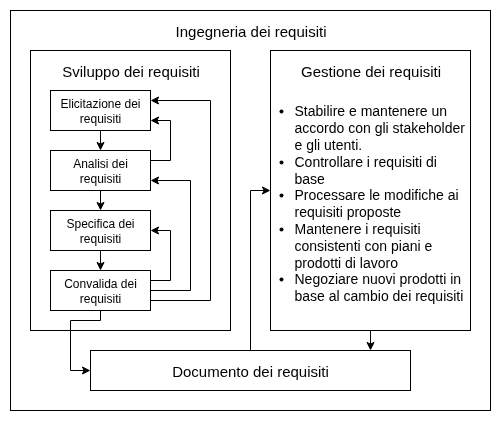
\includegraphics[width=0.8\linewidth]{Images/requirementsEngineering.png}
	\caption{Processi dell'ingegneria dei requisiti}
\end{figure}

%

\section{Use case}
L'utilizzo di \textbf{use case} è una tecnica non visuale per l'espressione dei requisiti funzionali di un sistema e la descrizione del sistema dal punto di vista dell'utenze, senza che questo sia cosciente degli eventi che avvengono al suo interno. Il software viene infatti visto come una black box della quale si descrive esclusivamente lo scambio di messaggi tra il sistema e le entità attive, dette \textbf{attori}. Il caso d'uso può presentare una "storia" che descrive una modalità di utilizzo da parte dell'utente. Per esempio, il programma di un ATM può essere descritto in due passaggi: \begin{enumerate}
	\item L'utente seleziona l'importo da prelevare e conferma la cifra.
	\item Il sistema eroga la cifra.
\end{enumerate}
\noindent Formalmente, gli use case hanno una struttura specifica; un insieme di campi che comprendono in primo luogo l'\textbf{ID del caso}, il \textbf{nome del caso}, una breve \textbf{descrizione dell'obiettivo} e gli \textbf{attori}. In una sezione sottostante è poi spiegato in termini semplici il \textbf{workflow principale}, ovvero l'istanza di utilizzo del software ideale, insieme ai \textbf{workflow secondari}, che mostrano il comportamento del sistema quando si devia dall'interazione ideale.\par
Principalmente, gli use case sono utili a documentare le scelte prese per rispettare i requisiti e presentare chiaramente il risultato agli stakeholder. Sono inoltre passati al team di sviluppo che progetterà l'applicativo, i quali potranno usarli come base per valutare la qualità del software.\newline

\noindent Per dare una visione ulteriormente chiara degli use case, è possibile ricondursi ad una forma grafica: gli \textbf{use case diagram}, composti da: \begin{itemize}
	\item \textbf{Attori}: Ruoli assunti dalle entità che interagiscono con il sistema. Si dividono a loro volta in \begin{itemize}
		\item \textbf{Primari}: Entità che hanno uno scopo raggiungibile grazie al sistema, come un utente che vuole comprare un prodotto su un sito di e-commerce.
		\item \textbf{Secondari}: Entità che producono qualcosa per il sistema, come il circuito di pagamento per l'elaborazione delle transazioni.
	\end{itemize}
	\noindent Possono essere anche organizzati in gerarchie e se trattano utenti sono rappresentati da stickmen.
	\item \textbf{Use case}: Ciò che gli attori possono eseguire con il sistema. Rappresentati da ellissi.
	\item \textbf{Relazioni}: Legami tra attori e use case. Rappresentate da archi tra le ellissi.
	\item \textbf{Confini del sistema}: Definisce l'insieme delle operazioni che il sistema può effettuare. Rappresentati da un rettangolo che contiene gli elementi precedenti.
\end{itemize}
\noindent La definizione dei confini del sistema è in particolar modo importante, poiché ha un grosso impatto sui requisiti funzionali; molti progetti sono falliti esattamente per questo problema.
\begin{figure}[h]
	\centering
	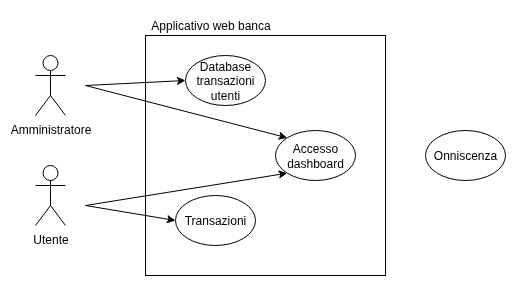
\includegraphics[width=0.7\linewidth]{Images/useCaseDiagram.png}
	\caption{Esempio di use case diagram}
\end{figure}

\noindent Altro concetto importante è quello di \textbf{scenario}; una sequenza ordinata di interazioni tra un sistema e gli attori che rappresenta una particolare istanza, e quindi un singolo cammino, di uno use case. Lavorare con degli scenari concreti è particolarmente utile perché possono essere utilizzati per il testing del codice. Naturalmente, un caso d'uso contiene più scenari e in questi termini possiamo formalmente definirli come insiemi di scenari che hanno in comune lo scopo finale dell'utente.\par
Prendiamo nuovamente in considerazione l'esempio dell'ATM; lo scenario ideale comprenderebbe: \begin{enumerate}
	\item L'utente esegue un tentativo di autenticazione.
	\item Il sistema verifica la correttezza dei dati e conferma l'accesso.
	\item L'utente inserisce l'importo da prelevare e conferma la cifra selezionata.
	\item Il sistema controlla che l'importo sia disponibile, ed in tal caso eroga il contante. 
\end{enumerate}
\noindent Tuttavia, è possibile che si verifichino altri scenari secondari, come l'inserimento di un pin errato, oppure la richiesta di prelevare più soldi di quanti sono disponibili sul conto. Queste istanze sono dette \textbf{deviazioni} e devono essere appropriatamente gestite e documentate. Quando ritornano nel workflow principale sono dette \textbf{semplici}, altrimenti si dicono \textbf{complesse}.\par
Inoltre, per la descrizione degli scenari è necessario specificare anche le \textbf{pre-condizioni}, i vincoli sullo stato corrente del sistema, e le \textbf{post-condizioni}, le condizioni che devono risultare vere quando lo use case termina con successo.\newline

\noindent Definiamo ora le possibili relazioni tra gli use case: \begin{itemize}
	\item \textbf{Inclusione}: Usato per associare un comportamento a più use case. Nella descrizione testuale si indica con $.include(caseName)$, mentre in quella grafica si scrive sopra l'arco $<<include>>$.
	\item \textbf{Estensione}: Usato per indicare un comportamento opzionale. Indicato via testo con $.extends(caseName)$ e $<<extends>>$ via grafica.
	\item \textbf{Generalizzazione}: Usato per la generalizzazione di più use case. Per esempio, se dei casi usano una stessa funzione di pagamento, si raggrupperanno in un altro use case più generale. Viceversa, si possono vedere i casi raggruppati come istanze più specifiche.
\end{itemize}
\noindent A supporto dei diagrammi degli use case è possibile usare dei tool appositi per fare degli \textbf{screen mockup}, ovvero degli schizzi dell'interfaccia utente per chiarirne il comportamento. Sono utili per aumentare la comprensibilità delle funzioni e a guidare lo svilippo del software dando un'idea di come dovrebbe risultare. Un esempio di questi tool sono quelli per la \textbf{GUI prototyping}.\par
Riassumendo, è bene scrivere use case brevi e semplici, con un buon compromesso fra astrazione e dettagli per la descrizione del comportamento di un sistema. Ne esistono diversi template equivalenti e sono molto utilizzati in ambito lavorativo. L'ambito in cui possono risultare meno utili è quello di sistemi dominati da requisiti non funzionali o con algoritmi complessi il cui funzionamento non necessita accoppiamento con interfaccia grafica.